% Volume III: Probability, Statistics, Information, and Causality
% Continuity note for Chapter 16.
% Previous dependencies: Chapter 13's probability spaces, random variables, distributions, random vectors, covariance, and independence; Chapter 14's named distribution families, Gaussian models, Poisson count models, and exponential-family likelihoods; Chapter 15's expectation, conditioning, Bayes updates, and decision rules as the surrounding course context for prediction under uncertainty.
% New durable concepts: sample mean; estimator fluctuation; weak law of large numbers; central limit theorem; standard error; convergence almost surely, in probability, in distribution, and in L^p; implication relationships among convergence modes; Markov, Chebyshev, and Hoeffding inequalities; sub-Gaussian tails; with-high-probability statements; sample-complexity bounds; high-dimensional norm concentration; near-orthogonality; thin-shell geometry; random projections; Johnson-Lindenstrauss distance preservation; curse and blessing of dimensionality.
% Forward hooks: Chapter 17 reuses standard errors, asymptotic normality, confidence intervals, hypothesis tests, risk estimates, and sample-complexity reasoning; Chapter 18 reuses concentration and high-dimensional probability when estimating entropy, KL divergence, mutual information, and Fisher geometry; later machine-learning and neuroscience chapters reuse random initialization, generalization bounds, neural population covariance, random features, embeddings, and dimensionality-reduction geometry.
% Notation commitments: Independent identically distributed variables are X_1,\ldots,X_n; common mean and variance are \mu=E[X_i] and \sigma^2=\operatorname{Var}(X_i); sample means are \bar X_n=n^{-1}\sum_{i=1}^n X_i; convergence is written X_n\to X, X_n\xrightarrow{p}X, X_n\xrightarrow{a.s.}X, X_n\xrightarrow{d}X, and X_n\to X in L^p; high-probability failure levels are \delta; deviations are \epsilon or t; high-dimensional vectors live in \mathbb R^d and random projections map \mathbb R^d to \mathbb R^k.
% Figure plan: four ImageGen raster figures under imagegen-figures/ch16-* are referenced: LLN/CLT sample means for 16.1; modes-of-convergence implication diagram for 16.2; concentration tail bounds for 16.3; high-dimensional geometry for 16.4.
\section{Chapter 16: Limit Theorems, Concentration, and High-Dimensional Probability}
\label{ch:limit-theorems-concentration-high-dimensional-probability}

Chapters 13 and 14 built probability models: outcome spaces, random variables, distributions, random vectors, covariance, and named families such as Bernoulli, Poisson, and Gaussian models. Chapter 15 turns those distributions into prediction, conditioning, and decision rules. Chapter 16 asks a different but equally practical question: what becomes predictable when the inputs themselves remain random?

The central answer is that randomness often has structure at scale. Averages stabilize. Properly standardized sums become nearly Gaussian. Tail probabilities can be bounded before we know the exact distribution. In high dimensions, random vectors are not chaotic clouds without geometry; their norms, angles, and projected distances obey surprisingly regular laws.

\paragraph{Chapter problem.}
Why do averages, empirical estimates, random embeddings, neural population vectors, and randomly initialized model quantities behave predictably even though each individual observation is random?

\paragraph{Section map.}
Section 16.1 develops the law of large numbers and central limit theorem for sample means. Section 16.2 distinguishes the main modes of convergence used to state probabilistic limits. Section 16.3 introduces concentration inequalities, which turn variance, boundedness, and independence into finite-sample guarantees. Section 16.4 explains the geometry of random vectors in high dimensions, including thin shells, near-orthogonality, and random projections.

\subsection{16.1 Law of large numbers and central limit theorem}

\paragraph{Motivating question.}
When repeated measurements are random, why does their average become stable, and why do the remaining fluctuations often look Gaussian?

\paragraph{Beginner setup.}
Suppose \(X_1,\ldots,X_n\) are repeated measurements of the same kind: coin-flip indicators, trial losses, spike counts in identical time windows, or noisy readings of a stimulus response. The sample mean is
\[
\bar X_n=\frac{1}{n}\sum_{i=1}^n X_i.
\]
If each \(X_i\) has mean \(\mu\), then \(\bar X_n\) is a natural estimate of \(\mu\). The smallest nontrivial example is a sequence of Bernoulli variables \(X_i\in\{0,1\}\), where \(X_i=1\) means heads or success. Then \(\bar X_n\) is the fraction of successes.

The problem solved by the law of large numbers is stability: it says that \(\bar X_n\) gets close to \(\mu\) as \(n\) grows. The problem solved by the central limit theorem is shape: it says that the remaining error, after scaling by its natural size, is approximately normal.

What to keep in mind: the observations do not stop being random. Averages become more predictable because independent positive and negative deviations cancel. The typical error of a sample mean is of order \(1/\sqrt n\), not \(1/n\). This slow square-root rate is why ten times more data does not give ten times smaller error.

\begin{figure}[htbp]
\centering
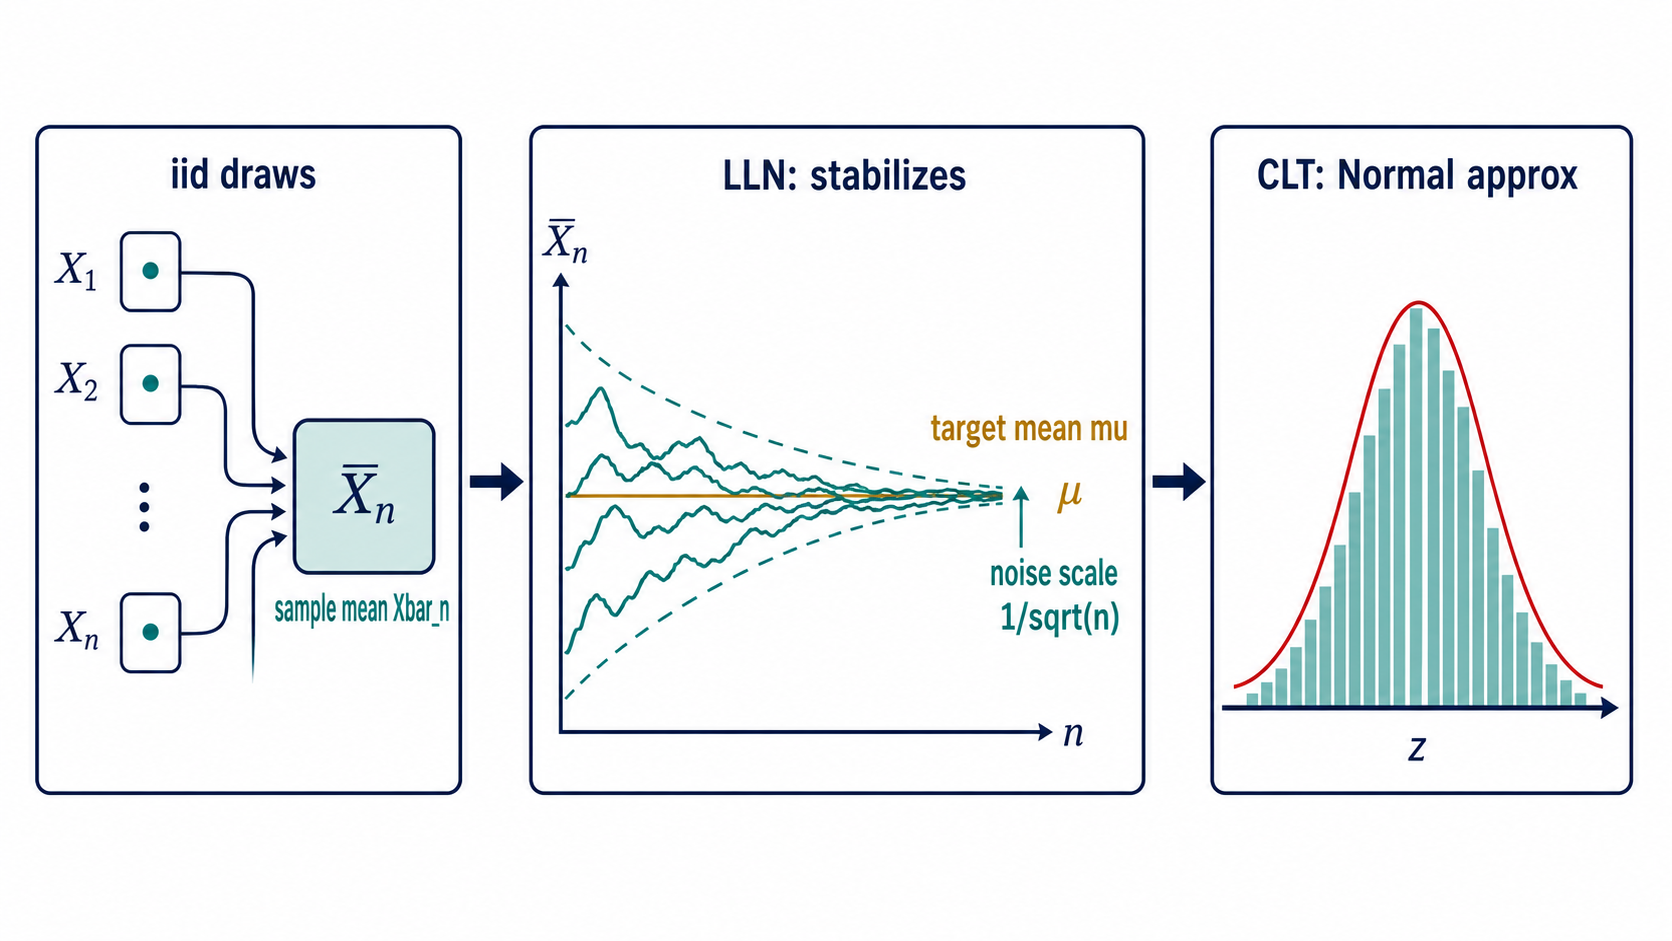
\includegraphics[width=0.98\linewidth]{imagegen-figures/ch16-lln-clt-sample-means.png}
\caption{The law of large numbers and central limit theorem describe two views of the same repeated-sampling process. The sample mean \(\bar X_n\) stabilizes near the true mean \(\mu\), while its standardized error \(\sqrt n(\bar X_n-\mu)/\sigma\) approaches a normal distribution under the usual iid finite-variance assumptions.}
\label{fig:ch16-lln-clt}
\end{figure}

\paragraph{Formal setup.}
Let \(X_1,X_2,\ldots\) be independent and identically distributed real-valued random variables with
\[
E[X_i]=\mu,\qquad \operatorname{Var}(X_i)=\sigma^2<\infty.
\]
The sample mean is
\[
\bar X_n=\frac{1}{n}\sum_{i=1}^n X_i.
\]
Its expectation and variance are
\[
E[\bar X_n]=\mu,
\qquad
\operatorname{Var}(\bar X_n)=\frac{\sigma^2}{n}.
\]
The weak law of large numbers says that for every \(\epsilon>0\),
\[
\boxed{\Pr(|\bar X_n-\mu|>\epsilon)\to0.}
\]
The central limit theorem says that, if \(0<\sigma^2<\infty\), then
\[
\boxed{\frac{\sqrt n(\bar X_n-\mu)}{\sigma}\xrightarrow{d}\mathcal N(0,1).}
\]
Equivalently, for large \(n\),
\[
\bar X_n\approx \mathcal N\!\left(\mu,\frac{\sigma^2}{n}\right).
\]
The quantity \(\sigma/\sqrt n\) is the \emph{standard error} of the sample mean.

\paragraph{Core intuition.}
Figure~\ref{fig:ch16-lln-clt} separates stabilization from fluctuation. The left and middle parts show many random observations being averaged. Individual paths wiggle, but the average is pulled toward \(\mu\). The right part shows the shape of the remaining standardized error. Once the error is measured in units of its standard deviation \(\sigma/\sqrt n\), its distribution often resembles the standard normal bell curve.

The law of large numbers is not saying that every finite average equals the mean. It is saying that large deviations become unlikely. The central limit theorem is not saying that the original data are normally distributed. It is saying that sums or averages of many small independent contributions are approximately normal after centering and scaling.

The iid and finite-variance assumptions matter. Strong dependence can prevent cancellation. Heavy-tailed variables with infinite variance may have non-Gaussian limits. Biased sampling can make the average converge to the wrong target. These are not technical details to memorize; they are the modeling assumptions that justify using data averages as reliable estimates.

This section uses Chapter 15's expectation as the target being estimated and Chapter 14's Gaussian distribution as the universal approximation for many standardized averages. It prepares Chapter 17's confidence intervals, standard errors, and asymptotic likelihood approximations.

\paragraph{Main theorem: LLN by Chebyshev and CLT by local expansion.}
Under the iid finite-variance assumptions above, \(\bar X_n\xrightarrow{p}\mu\). If additionally \(0<\sigma^2<\infty\), then
\[
\sqrt n(\bar X_n-\mu)/\sigma \xrightarrow{d}\mathcal N(0,1).
\]

\emph{Proof sketch for the weak LLN.}
The sample mean has variance \(\sigma^2/n\). Chebyshev's inequality gives
\[
\Pr(|\bar X_n-\mu|>\epsilon)
\leq
\frac{\operatorname{Var}(\bar X_n)}{\epsilon^2}
=
\frac{\sigma^2}{n\epsilon^2}.
\]
The right-hand side goes to \(0\). The mechanism is transparent: averaging divides the variance by \(n\), so the probability of a fixed-size error must shrink.

\emph{Proof sketch for the CLT mechanism.}
Assume for simplicity that \(E[X_i]=0\) and \(\operatorname{Var}(X_i)=1\). Let
\[
S_n=\frac{X_1+\cdots+X_n}{\sqrt n}.
\]
For many well-behaved variables, the moment-generating function of one scaled term has the local expansion
\[
E[e^{tX_i/\sqrt n}]
=1+\frac{t^2}{2n}+o(1/n),
\]
because the mean term is \(0\) and the variance term is \(1\). Independence gives
\[
E[e^{tS_n}]
=\left(E[e^{tX_i/\sqrt n}]\right)^n
\approx
\left(1+\frac{t^2}{2n}\right)^n
\to e^{t^2/2}.
\]
The function \(e^{t^2/2}\) is the moment-generating function of \(\mathcal N(0,1)\). The algebra says that many small independent effects multiply in transform space and become the exponential quadratic signature of a Gaussian.

\paragraph{Worked examples.}
\emph{Small numerical example.}
Let \(X_i\sim\mathrm{Bernoulli}(0.6)\), independently. Then \(\mu=0.6\) and \(\sigma^2=0.6(0.4)=0.24\). For \(n=100\),
\[
\operatorname{sd}(\bar X_{100})=\frac{\sqrt{0.24}}{10}\approx0.049.
\]
The CLT approximation says
\[
\bar X_{100}\approx\mathcal N(0.6,0.049^2).
\]
The probability that the observed success fraction exceeds \(0.70\) is approximately
\[
\Pr\!\left(Z>\frac{0.70-0.60}{0.049}\right)
=\Pr(Z>2.04)\approx0.021.
\]

\emph{Neuroscience example.}
Suppose a neuron has trial-to-trial spike count \(X_i\) in a fixed window with mean \(8\) spikes and variance \(12\). The average spike count across \(n=48\) repeated trials has standard error
\[
\sqrt{12/48}=0.5.
\]
The sample mean is still random, but a typical error is about half a spike. If a second stimulus changes the mean response by \(3\) spikes, that difference is large relative to this standard error. If the change is \(0.2\) spikes, many more trials or a different analysis may be needed.

\emph{Machine-learning example.}
Let \(X_i=\ell(f_\theta(x_i),y_i)\) be the loss of a fixed model on a randomly sampled data point. The population risk is \(E[X_i]\), and the test-set average \(\bar X_n\) estimates it. The LLN explains why a large independent test set gives a stable risk estimate. The CLT explains why reported test error often comes with an uncertainty of order \(1/\sqrt n\).

\paragraph{ML/DL/neuroscience connections.}
For empirical risk, \(X_i\) is a loss and \(\bar X_n\) is the average test or training loss. For decoding accuracy, \(X_i\) can be a correct/incorrect indicator and \(\bar X_n\) is accuracy. For neural data, \(X_i\) may be a spike count, a calcium response, or a projected population response on trial \(i\). The LLN maps repeated trials to stable estimates of means. The CLT maps remaining estimator noise to approximate Gaussian uncertainty, which Chapter 17 turns into intervals, tests, and likelihood approximations.

\paragraph{Exercises.}
\begin{enumerate}[label=\textbf{16.1.\arabic*.}, leftmargin=*]
\item \textbf{Mechanical.} Let \(X_i\) be iid with mean \(5\) and variance \(9\). Compute \(E[\bar X_{36}]\), \(\operatorname{Var}(\bar X_{36})\), and the standard error of \(\bar X_{36}\).
\item \textbf{Proof or derivation.} Prove that \(\operatorname{Var}(\bar X_n)=\sigma^2/n\) when \(X_1,\ldots,X_n\) are independent with common variance \(\sigma^2\).
\item \textbf{Numerical/computational.} For iid Bernoulli\((0.5)\) observations with \(n=400\), use the CLT to approximate \(\Pr(|\bar X_n-0.5|>0.05)\). State the standard error you used.
\item \textbf{Interpretation.} In a neural experiment, doubling the number of repeated trials does not halve the standard error of the mean response. What factor does it change by, and why?
\item \textbf{Debug the misconception.} A student says, "The CLT means the data must be normal if the sample size is large." Correct the statement using the distinction between individual observations and standardized sample means.
\end{enumerate}

\subsection{16.2 Modes of convergence}

\paragraph{Motivating question.}
When we write that random variables \(X_n\) converge to \(X\), what exactly is converging: sample paths, error probabilities, distributions, or moments?

\paragraph{Beginner setup.}
In ordinary calculus, a sequence \(a_n\) either approaches a number \(a\) or it does not. Random variables are more subtle because each \(X_n\) is a function of the outcome \(\omega\). There are several reasonable meanings of "approaches." A simulated estimator may settle on almost every run. Its probability of being far from the target may go to zero. Its distribution may approach a limiting distribution. Its mean squared error may go to zero.

The smallest nontrivial example is
\[
X_n=Z+\frac{1}{n},
\]
where \(Z\) is one random variable. For every outcome \(\omega\), \(X_n(\omega)\to Z(\omega)\). This is a very strong kind of convergence because the sample path itself settles.

Modes of convergence solve a communication problem. The law of large numbers, central limit theorem, stochastic optimization guarantees, and finite-sample bounds all need different kinds of limiting statements. Saying only "converges" hides the important part.

What to keep in mind: stronger convergence gives more information. Almost sure convergence controls individual sample paths. Convergence in probability controls the probability of being wrong by more than \(\epsilon\). Convergence in distribution controls only the limiting law. \(L^p\) convergence controls average \(p\)-th power error.

\begin{figure}[htbp]
\centering
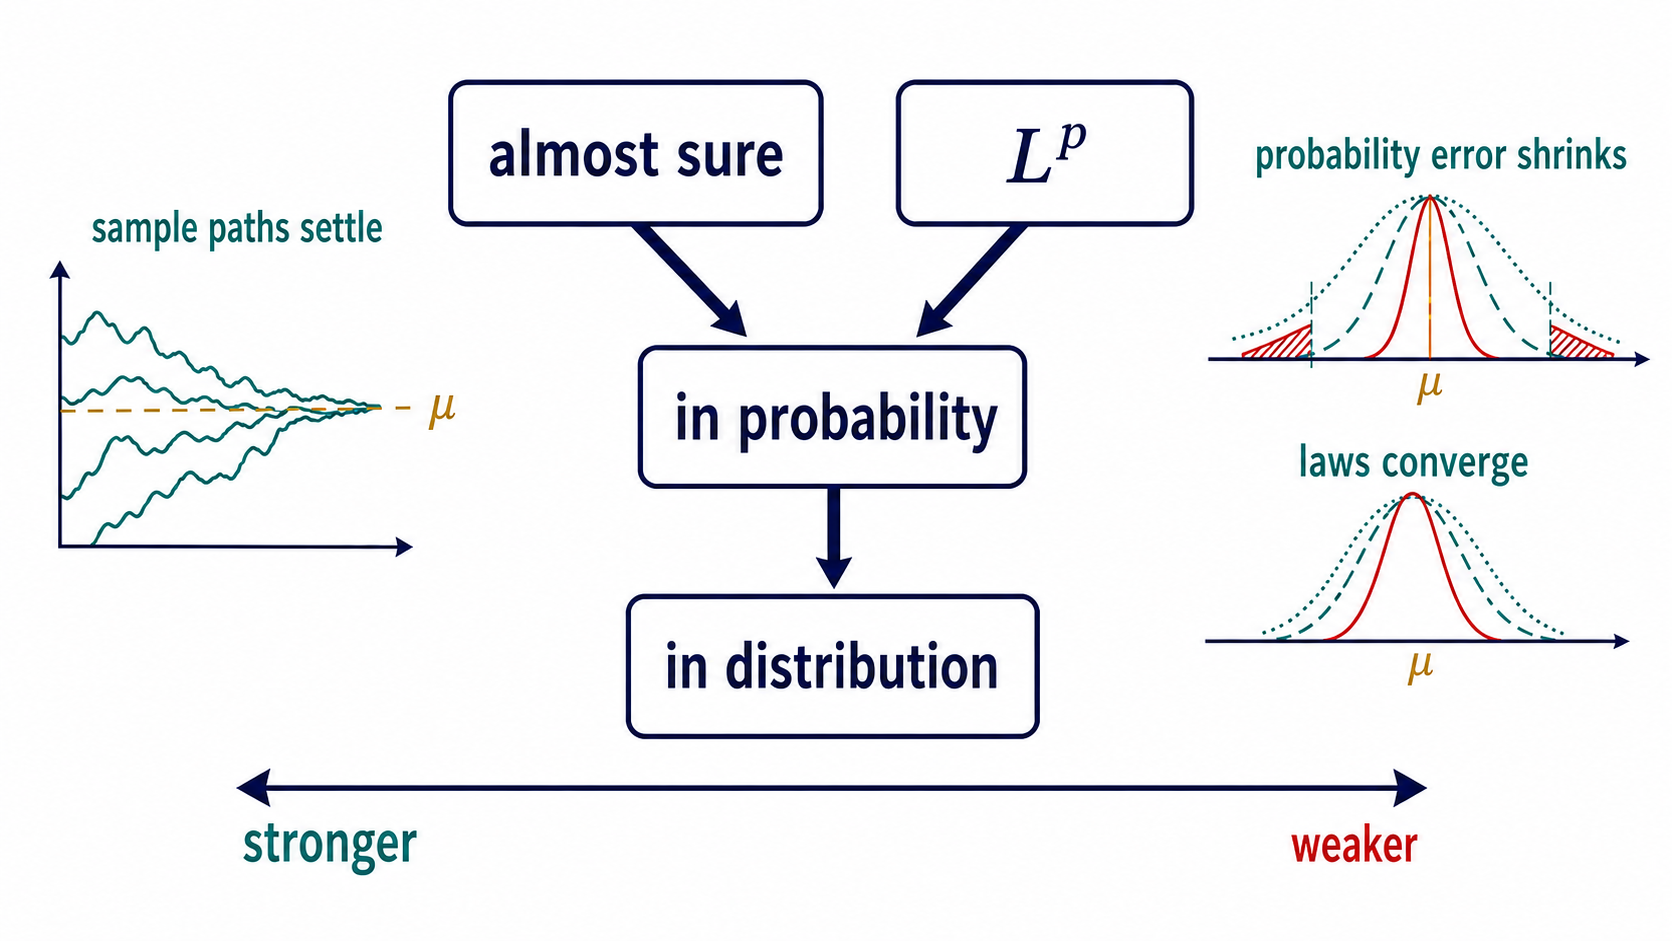
\includegraphics[width=0.98\linewidth]{imagegen-figures/ch16-modes-of-convergence.png}
\caption{Different modes of convergence answer different questions. Almost sure convergence and \(L^p\) convergence each imply convergence in probability, and convergence in probability implies convergence in distribution. The reverse implications generally require extra assumptions.}
\label{fig:ch16-modes-convergence}
\end{figure}

\paragraph{Formal setup.}
Let \(X_1,X_2,\ldots\) and \(X\) be random variables on a common probability space unless convergence in distribution is being discussed. The four main modes are:
\[
\boxed{X_n\xrightarrow{a.s.}X
\quad\Longleftrightarrow\quad
\Pr\{\omega:X_n(\omega)\to X(\omega)\}=1.}
\]
\[
\boxed{X_n\xrightarrow{p}X
\quad\Longleftrightarrow\quad
\text{for every }\epsilon>0,\
\Pr(|X_n-X|>\epsilon)\to0.}
\]
\[
\boxed{X_n\xrightarrow{d}X
\quad\Longleftrightarrow\quad
F_{X_n}(t)\to F_X(t)\text{ at every continuity point }t\text{ of }F_X.}
\]
\[
\boxed{X_n\to X\text{ in }L^p
\quad\Longleftrightarrow\quad
E[|X_n-X|^p]\to0.}
\]
Here \(p\geq1\), and \(F_Y(t)=\Pr(Y\leq t)\) is the cumulative distribution function of \(Y\). The most common case in estimation is \(L^2\) convergence, also called mean-square convergence.

The implication structure used most often is
\[
X_n\xrightarrow{a.s.}X\Longrightarrow X_n\xrightarrow{p}X\Longrightarrow X_n\xrightarrow{d}X,
\]
and
\[
X_n\to X\text{ in }L^p\Longrightarrow X_n\xrightarrow{p}X.
\]
If \(X\) is a constant, convergence in distribution to \(X\) also implies convergence in probability to \(X\).

\paragraph{Core intuition.}
Figure~\ref{fig:ch16-modes-convergence} is an implication diagram, not a ranking of importance. Almost sure convergence asks whether each run eventually settles, except possibly on a probability-zero set of strange outcomes. Convergence in probability asks whether the chance of a noticeable error becomes small. Convergence in distribution asks whether histograms or CDFs approach a limiting shape, which need not mean collapse to a point mass. \(L^p\) convergence asks whether average error magnitude goes to zero.

A common beginner mistake is to confuse convergence in distribution with convergence of paired values. If \(X_n\) has the same distribution as \(X\), then \(X_n\) may converge in distribution to \(X\) even if \(X_n(\omega)\) does not get close to \(X(\omega)\) on the same outcome. Distributional convergence compares laws, not sample-by-sample errors.

Another mistake is to treat almost sure convergence as meaning "sure for every possible outcome." The phrase "almost" matters: exceptions may exist, but their probability is zero. This is the same probability-zero idea introduced for continuous distributions in Chapter 13.

This section clarifies the statements used in Section 16.1. The weak law is convergence in probability. Strong laws, when available, are almost sure statements. The CLT is convergence in distribution. Chapter 17 will use all three: consistency often means convergence in probability, asymptotic normality is convergence in distribution, and mean-square error is an \(L^2\) quantity.

\paragraph{Main theorem: basic implication chain.}
If \(X_n\xrightarrow{a.s.}X\), then \(X_n\xrightarrow{p}X\). If \(X_n\to X\) in \(L^p\), then \(X_n\xrightarrow{p}X\). If \(X_n\xrightarrow{p}X\), then \(X_n\xrightarrow{d}X\).

\emph{Proof sketch.}
For almost sure convergence, define the error events
\[
A_{n,\epsilon}=\{|X_n-X|>\epsilon\}.
\]
If \(X_n(\omega)\to X(\omega)\), then for that \(\omega\), the event \(A_{n,\epsilon}\) eventually stops occurring. To make this rigorous, define the tail event
\[
B_{N,\epsilon}=\bigcup_{n\geq N}A_{n,\epsilon},
\]
the event that an \(\epsilon\)-sized error happens at least once after time \(N\). The events \(B_{N,\epsilon}\) decrease as \(N\) grows, and
\[
\bigcap_{N=1}^{\infty}B_{N,\epsilon}
\]
is the event that \(\epsilon\)-sized errors occur infinitely often. Almost sure convergence implies this event has probability \(0\). By continuity of probability for decreasing events,
\[
\Pr(B_{N,\epsilon})\downarrow0.
\]
For every \(n\geq N\), \(A_{n,\epsilon}\subseteq B_{N,\epsilon}\), so
\[
\Pr(A_{n,\epsilon})\leq \Pr(B_{N,\epsilon}).
\]
Taking \(N\) large makes the right-hand side small for all later \(n\), hence \(\Pr(|X_n-X|>\epsilon)\to0\). Eventual sample-path settling rules out persistent error probability.

For \(L^p\) convergence, Markov's inequality applied to the nonnegative random variable \(|X_n-X|^p\) gives
\[
\Pr(|X_n-X|>\epsilon)
=
\Pr(|X_n-X|^p>\epsilon^p)
\leq
\frac{E[|X_n-X|^p]}{\epsilon^p}.
\]
The right-hand side goes to \(0\), so \(X_n\xrightarrow{p}X\).

For convergence in probability implying convergence in distribution, look at CDFs. If \(X_n\) is within \(\epsilon\) of \(X\) with high probability, then the event \(\{X\leq t-\epsilon\}\) is mostly contained in \(\{X_n\leq t\}\), and \(\{X_n\leq t\}\) is mostly contained in \(\{X\leq t+\epsilon\}\). Therefore
\[
F_X(t-\epsilon)-\Pr(|X_n-X|>\epsilon)
\leq F_{X_n}(t)
\leq F_X(t+\epsilon)+\Pr(|X_n-X|>\epsilon).
\]
Let \(n\to\infty\), then \(\epsilon\downarrow0\) at continuity points of \(F_X\). The CDFs converge.

\paragraph{Worked examples.}
\emph{Small symbolic example.}
Let \(X_n=Z+1/n\), where \(E[|Z|^2]<\infty\). Then \(X_n\to Z\) almost surely because \(1/n\to0\) for every outcome. Also
\[
E[|X_n-Z|^2]=E[(1/n)^2]=1/n^2\to0,
\]
so \(X_n\to Z\) in \(L^2\), hence in probability and in distribution.

\emph{Convergence in distribution without paired closeness.}
Let \(Z\sim\mathcal N(0,1)\), and define
\[
X_n=
\begin{cases}
Z, & n\text{ even},\\
-Z, & n\text{ odd}.
\end{cases}
\]
Every \(X_n\) has the standard normal distribution, so \(X_n\xrightarrow{d}Z\). But \(X_n\) does not converge in probability to \(Z\), because for odd \(n\),
\[
|X_n-Z|=|-Z-Z|=2|Z|,
\]
which is not small with high probability. The laws match, but the paired values do not settle.

\emph{Machine-learning example.}
Let \(\hat R_n(\theta)\) be empirical risk for a fixed model \(\theta\), and let \(R(\theta)=E[\ell_\theta(X,Y)]\). A law of large numbers says
\[
\hat R_n(\theta)\xrightarrow{p}R(\theta).
\]
This means the probability that the empirical risk is more than \(\epsilon\) away from the true risk goes to zero. It does not by itself describe the limiting shape of the error; a CLT would add that.

\emph{Stochastic optimization example.}
If a stochastic-gradient method produces random parameters \(\Theta_n\), then saying \(\Theta_n\xrightarrow{p}\theta^\star\) means the optimizer is close to \(\theta^\star\) with high probability. Saying \(E[\|\Theta_n-\theta^\star\|^2]\to0\) is stronger: it controls mean squared distance, not just the probability of a large miss.

\paragraph{ML/DL/neuroscience connections.}
In statistical learning, consistency is usually convergence in probability or almost sure convergence of an estimator to a target. Asymptotic normality is convergence in distribution of a standardized estimator. Mean-square convergence describes prediction error or parameter error in \(L^2\). In neuroscience, trial-averaged responses may converge in probability to mean tuning curves, while empirical covariance matrices may converge in operator norm or Frobenius \(L^2\)-type measures. The chosen convergence mode states exactly what reliability claim is being made.

\paragraph{Exercises.}
\begin{enumerate}[label=\textbf{16.2.\arabic*.}, leftmargin=*]
\item \textbf{Mechanical.} Write the definition of \(X_n\xrightarrow{p}X\). Then specialize it to the statement \(\bar X_n\xrightarrow{p}\mu\).
\item \textbf{Proof or derivation.} Use Markov's inequality to prove that \(L^2\) convergence implies convergence in probability.
\item \textbf{Numerical/computational.} Suppose \(E[(\hat\theta_n-\theta)^2]=4/n\). Use Chebyshev or Markov's inequality to bound \(\Pr(|\hat\theta_n-\theta|>0.2)\) when \(n=400\).
\item \textbf{Interpretation.} A training run produces random validation accuracy \(A_n\). What is the difference between saying \(A_n\xrightarrow{p}0.92\) and saying \(A_n\xrightarrow{d}\mathcal N(0.92,0.01^2)\)?
\item \textbf{Debug the misconception.} A student says, "If two random variables have the same distribution, they must be close." Use the example \(Z\) and \(-Z\) for \(Z\sim\mathcal N(0,1)\) to correct the misconception.
\end{enumerate}

\subsection{16.3 Concentration inequalities}

\paragraph{Motivating question.}
How can we guarantee that a random estimate is close to its mean with high probability before we know its exact distribution?

\paragraph{Beginner setup.}
A concentration inequality is a tail bound. It controls probabilities such as
\[
\Pr(|Z-E[Z]|\geq t)
\]
using limited information about \(Z\): nonnegativity, variance, bounded range, independence, or sub-Gaussian behavior. These inequalities are finite-sample tools. They do not wait for \(n\to\infty\); they say how large a deviation can be at a given sample size.

The smallest nontrivial example is a sample mean of bounded variables. If \(X_i\in[0,1]\) are independent with mean \(\mu\), then Hoeffding's inequality says
\[
\Pr(|\bar X_n-\mu|\geq\epsilon)\leq 2e^{-2n\epsilon^2}.
\]
This turns a target accuracy \(\epsilon\) and failure probability \(\delta\) into a required sample size.

What to keep in mind: concentration is about the tail event, not just about a typical value. A statement that holds "with high probability" usually means it fails with probability at most \(\delta\), where \(\delta\) is chosen in advance. The bound may be conservative, but it is often distribution-free within its assumptions.

\begin{figure}[htbp]
\centering
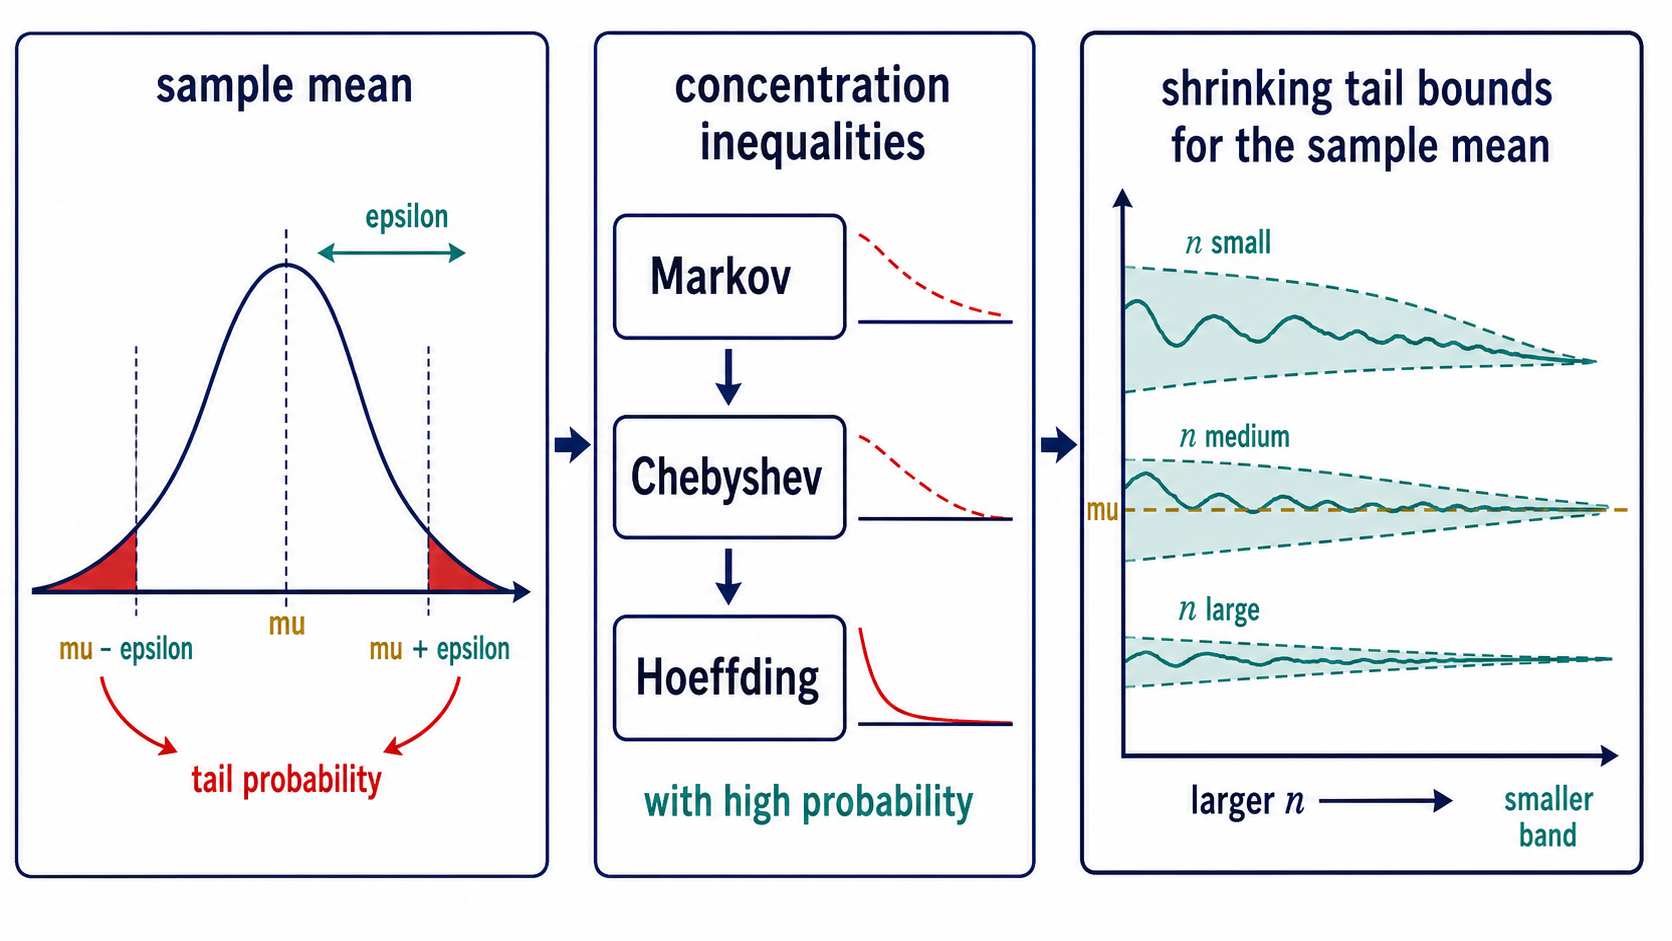
\includegraphics[width=0.98\linewidth]{imagegen-figures/ch16-concentration-tail-bounds.png}
\caption{Concentration inequalities bound the probability of large deviations. Markov uses nonnegativity, Chebyshev uses variance, and Hoeffding uses independence plus bounded observations. For sample means, the high-probability band shrinks as \(n\) grows.}
\label{fig:ch16-concentration}
\end{figure}

\paragraph{Formal setup.}
The general object is a real random variable \(Z\) and a tail probability
\[
\Pr(Z\geq a)
\quad\text{or}\quad
\Pr(|Z-E[Z]|\geq t).
\]
Three core inequalities are:
\[
\boxed{\text{Markov: if }Z\geq0,\quad \Pr(Z\geq a)\leq \frac{E[Z]}{a},\quad a>0.}
\]
\[
\boxed{\text{Chebyshev: if }E[Z]=\mu,\ \operatorname{Var}(Z)<\infty,\quad
\Pr(|Z-\mu|\geq t)\leq\frac{\operatorname{Var}(Z)}{t^2}.}
\]
\[
\boxed{\text{Hoeffding: if }X_i\in[a,b]\text{ iid and }E[X_i]=\mu,\quad
\Pr(|\bar X_n-\mu|\geq\epsilon)\leq2\exp\!\left(-\frac{2n\epsilon^2}{(b-a)^2}\right).}
\]
A mean-zero random variable \(Y\) is \(\sigma\)-sub-Gaussian if
\[
E[e^{\lambda Y}]\leq e^{\lambda^2\sigma^2/2}
\quad\text{for every }\lambda\in\mathbb R.
\]
Sub-Gaussian variables have Gaussian-like tails:
\[
\Pr(|Y|\geq t)\leq2e^{-t^2/(2\sigma^2)}.
\]

\paragraph{Core intuition.}
Figure~\ref{fig:ch16-concentration} shows the idea geometrically. A tail event is the shaded region far from the mean. Markov gives a crude one-sided control when the variable is nonnegative: if the average amount is small, the chance of being huge cannot be too large. Chebyshev improves this by using variance: if a variable has small spread, it cannot often be many standard deviations away. Hoeffding is sharper for bounded independent observations because each observation has limited ability to move the average.

The key difference from the CLT is that concentration inequalities are guarantees, not approximations. The CLT may give an accurate normal approximation for large \(n\), but Hoeffding gives a valid upper bound for every \(n\) under boundedness and independence. The price is conservativeness.

Common misconceptions: first, a tail bound is not usually an exact probability. It is an upper bound. Second, "with high probability" does not mean certainty; it means the failure probability has been controlled. Third, using Hoeffding without boundedness or independence is a modeling error. Heavy-tailed losses, temporal dependence, and adaptive data collection require different tools.

This section strengthens the LLN. Instead of only saying that the error probability goes to zero, it gives explicit rates. Chapter 17 will reuse these rates for confidence intervals and risk estimation. Machine-learning theory uses the same style to relate empirical performance to population performance.

\paragraph{Main derivation: from exponential Markov to Hoeffding.}
Markov's inequality is the starting point. For any nonnegative random variable \(W\) and \(a>0\),
\[
\Pr(W\geq a)\leq\frac{E[W]}{a}.
\]
To bound an upper tail for a centered sum \(S_n=\sum_{i=1}^n(X_i-\mu)\), choose \(W=e^{\lambda S_n}\), where \(\lambda>0\). Then
\[
\Pr(S_n\geq n\epsilon)
=\Pr(e^{\lambda S_n}\geq e^{\lambda n\epsilon})
\leq e^{-\lambda n\epsilon}E[e^{\lambda S_n}].
\]
Independence factors the exponential moment:
\[
E[e^{\lambda S_n}]
=\prod_{i=1}^n E[e^{\lambda(X_i-\mu)}].
\]
If each \(X_i\in[a,b]\), Hoeffding's lemma gives
\[
E[e^{\lambda(X_i-\mu)}]\leq
\exp\!\left(\frac{\lambda^2(b-a)^2}{8}\right).
\]
Therefore
\[
\Pr(S_n\geq n\epsilon)
\leq
\exp\!\left(-\lambda n\epsilon+\frac{n\lambda^2(b-a)^2}{8}\right).
\]
Choose the best \(\lambda\), namely
\[
\lambda=\frac{4\epsilon}{(b-a)^2}.
\]
Substituting gives
\[
\Pr(\bar X_n-\mu\geq\epsilon)
\leq
\exp\!\left(-\frac{2n\epsilon^2}{(b-a)^2}\right).
\]
The same argument applied to \(-S_n\) bounds the lower tail. Adding the two tail probabilities gives Hoeffding's two-sided inequality.

\paragraph{Worked examples.}
\emph{Sample-complexity example.}
Suppose \(X_i\in[0,1]\) are independent losses and \(\bar X_n\) estimates the true risk \(\mu\). To guarantee
\[
\Pr(|\bar X_n-\mu|\geq0.05)\leq0.05,
\]
Hoeffding requires
\[
2e^{-2n(0.05)^2}\leq0.05.
\]
Taking logarithms,
\[
n\geq \frac{\log(2/0.05)}{2(0.05)^2}
=\frac{\log 40}{0.005}
\approx738.
\]
So about \(738\) independent bounded test examples are enough for this conservative guarantee.

\emph{Chebyshev example.}
Let \(Z\) be an estimator with mean \(\theta\) and variance \(0.01\). Then
\[
\Pr(|Z-\theta|\geq0.2)\leq \frac{0.01}{0.2^2}=0.25.
\]
This bound may be loose, but it uses only the variance.

\emph{Neuroscience example.}
Let \(X_i\in[0,1]\) indicate whether a neuron fired at least one spike on trial \(i\). The firing probability is \(p=E[X_i]\). If \(n=1000\), Hoeffding gives
\[
\Pr(|\bar X_n-p|\geq0.05)\leq2e^{-2(1000)(0.05)^2}
=2e^{-5}\approx0.0135.
\]
Thus the empirical firing probability is within \(0.05\) of the true trial probability with probability at least \(0.9865\), under independent repeated trials.

\emph{Deep-learning example.}
If validation losses are clipped to \([0,1]\), Hoeffding can bound the difference between validation loss and population loss for a fixed trained model. The random variable is the validation loss on a random example, the sample mean is the validation average, and the failure probability \(\delta\) quantifies how often the validation estimate could be off by more than \(\epsilon\).

\paragraph{ML/DL/neuroscience connections.}
Concentration turns empirical averages into reliability statements. In ML, bounded loss concentration supports test-set uncertainty, ablation comparisons, and simple generalization arguments for fixed model classes. In deep learning, sub-Gaussian and related tail assumptions appear when analyzing random initialization, stochastic gradients, and random features. In neuroscience, concentration quantifies how many trials are needed to estimate firing probabilities, tuning-curve means, decoding accuracy, or covariance entries within a desired tolerance. The mathematical map is direct: observations become \(X_i\), the empirical quantity is \(\bar X_n\), and the tail bound controls the probability of a misleading deviation.

\paragraph{Exercises.}
\begin{enumerate}[label=\textbf{16.3.\arabic*.}, leftmargin=*]
\item \textbf{Mechanical.} State Markov's inequality and Chebyshev's inequality. For each one, list the assumption it requires.
\item \textbf{Proof or derivation.} Derive Chebyshev's inequality by applying Markov's inequality to \((Z-\mu)^2\).
\item \textbf{Numerical/computational.} Use Hoeffding's inequality for \(X_i\in[0,1]\) to find a sufficient \(n\) so that \(\Pr(|\bar X_n-\mu|\geq0.02)\leq0.01\).
\item \textbf{Interpretation.} Why might a Hoeffding bound be valid but much more conservative than a CLT approximation for the same sample mean?
\item \textbf{Debug the misconception.} A student applies Hoeffding to unbounded Gaussian observations. Explain which assumption is violated and name one inequality from this section that can still be used if the variance is finite.
\end{enumerate}

\subsection{16.4 High-dimensional geometry}

\paragraph{Motivating question.}
Why do random vectors in high dimensions have predictable norms, nearly right angles, and useful low-dimensional projections?

\paragraph{Beginner setup.}
A high-dimensional random vector is a vector with many random coordinates:
\[
X=(X_1,\ldots,X_d)\in\mathbb R^d.
\]
In neural population analysis, \(d\) might be the number of recorded neurons. In representation learning, \(d\) might be an embedding dimension. In random initialization, \(d\) might be fan-in or parameter dimension.

The smallest useful example is a standard Gaussian vector
\[
X\sim\mathcal N(0,I_d).
\]
Each coordinate has mean \(0\) and variance \(1\), so
\[
\|X\|^2=X_1^2+\cdots+X_d^2.
\]
The expected squared norm is \(d\), so the norm is typically near \(\sqrt d\). More surprisingly, the relative fluctuation of \(\|X\|^2\) shrinks as \(d\) grows.

High-dimensional probability solves a geometry problem. Our low-dimensional intuition says random points should spread everywhere in a ball. In high dimensions, most Gaussian mass lies in a thin shell, random directions are nearly orthogonal, and random projections can preserve many pairwise distances. These facts are both a curse and a blessing: data become sparse and distances can lose contrast, but random representations can also be stable and surprisingly informative.

\begin{figure}[htbp]
\centering
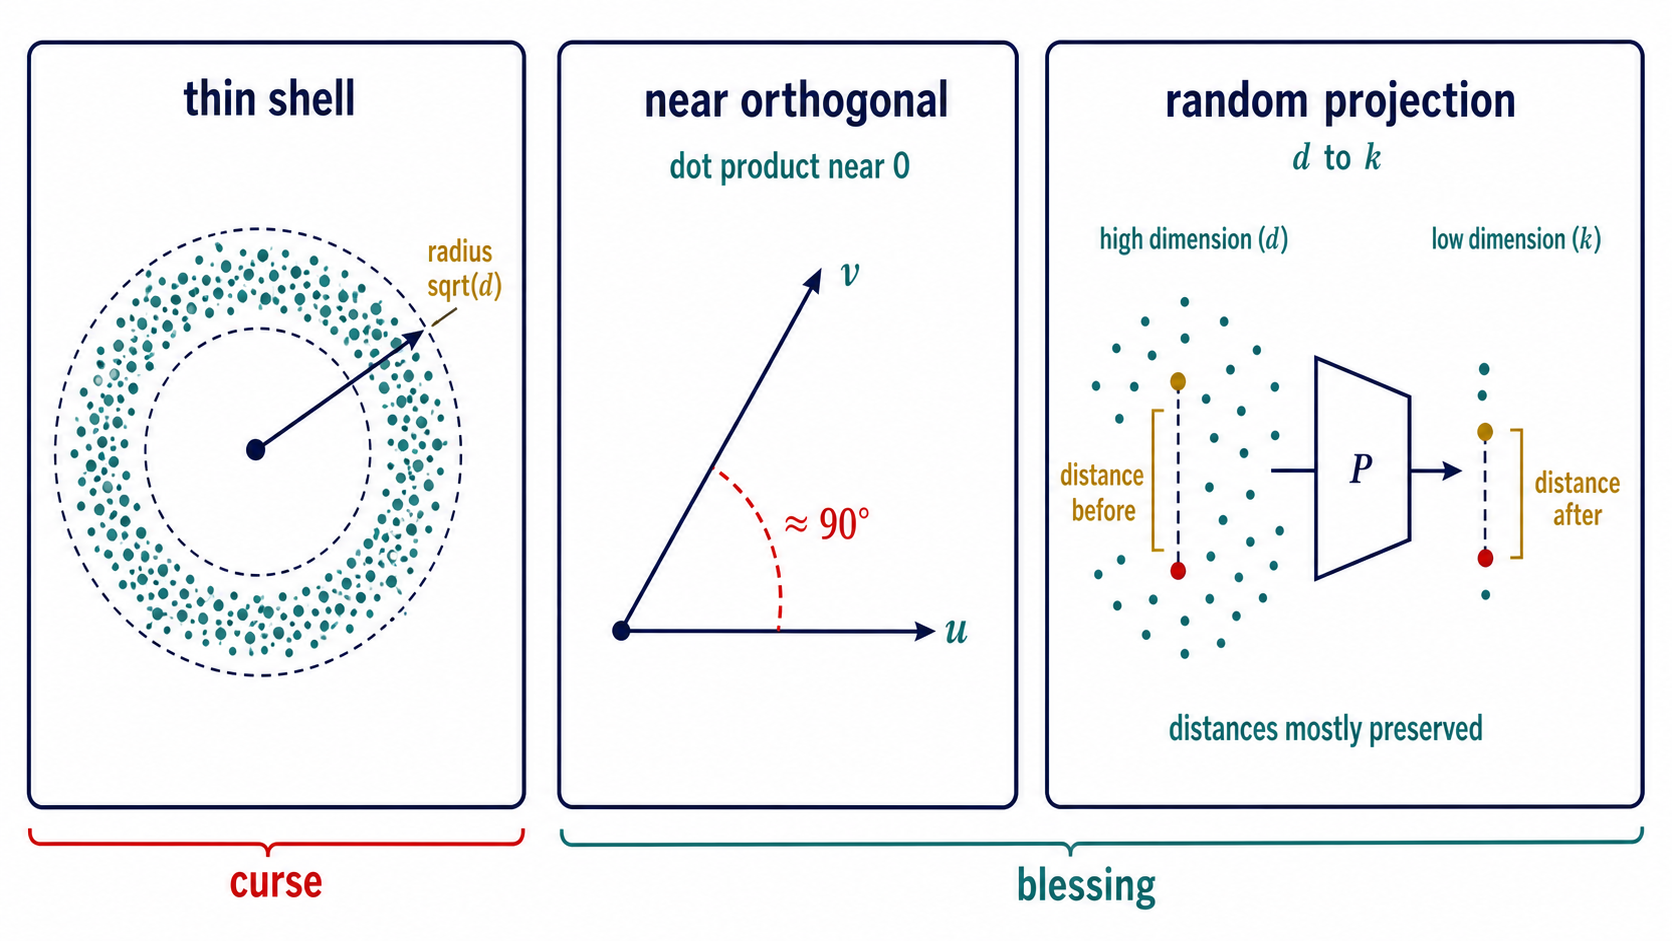
\includegraphics[width=0.98\linewidth]{imagegen-figures/ch16-high-dimensional-geometry.png}
\caption{High-dimensional random geometry has regular structure. Gaussian vectors concentrate in a thin shell of radius about \(\sqrt d\), independent random directions are nearly orthogonal, and random projections from \(d\) dimensions to \(k\) dimensions can preserve many pairwise distances when \(k\) is large enough.}
\label{fig:ch16-high-dimensional-geometry}
\end{figure}

\paragraph{Formal setup.}
Let \(X\sim\mathcal N(0,I_d)\), so \(X_1,\ldots,X_d\) are iid \(\mathcal N(0,1)\). Then
\[
\|X\|^2=\sum_{j=1}^d X_j^2,
\qquad
E[\|X\|^2]=d,
\qquad
\operatorname{Var}(\|X\|^2)=2d.
\]
The relative variance is
\[
\operatorname{Var}\!\left(\frac{\|X\|^2}{d}\right)=\frac{2}{d}.
\]
So \(\|X\|^2/d\) concentrates around \(1\).

For two independent random unit vectors \(U,V\) uniformly distributed on the sphere in \(\mathbb R^d\),
\[
E[U^\top V]=0,
\qquad
\operatorname{Var}(U^\top V)=\frac{1}{d}.
\]
Thus random directions have dot products typically of size \(1/\sqrt d\).

A random projection is a linear map \(A:\mathbb R^d\to\mathbb R^k\), often scaled so that distances are preserved on average:
\[
f(x)=\frac{1}{\sqrt k}Ax,
\]
where the entries of \(A\) may be independent signs or standard Gaussian entries. The Johnson-Lindenstrauss principle says that for \(m\) fixed points, \(k\) on the order of \(\log(m)/\epsilon^2\) is enough to preserve all pairwise distances within a factor \(1\pm\epsilon\), with high probability:
\[
\boxed{(1-\epsilon)\|x_i-x_j\|^2
\leq
\|f(x_i)-f(x_j)\|^2
\leq
(1+\epsilon)\|x_i-x_j\|^2.}
\]

\paragraph{Core intuition.}
Figure~\ref{fig:ch16-high-dimensional-geometry} shows three linked facts. First, a high-dimensional Gaussian does not fill the ball uniformly. Most mass lies near a shell because the squared norm is a sum of many independent coordinate contributions, and sums concentrate. Second, random directions have little alignment because there are many dimensions in which positive and negative coordinate products cancel. Third, a random projection can preserve distances because each projected distance is an average of many small random contributions.

The curse of dimensionality is real: grids become impossible, volumes behave strangely, nearest-neighbor distances can become less informative, and estimating densities requires enormous data. The blessing of dimensionality is also real: random vectors become regular, random features can be nearly orthogonal, high-dimensional codes can separate patterns, and concentration makes some randomized algorithms reliable.

Common misconceptions: high-dimensional does not mean "anything can happen." Many random quantities are more tightly controlled in high dimensions than in low dimensions. Also, near-orthogonality does not mean independence in every sense; it means inner products are small for many random or isotropic directions. Finally, random projection does not preserve every possible vector in \(\mathbb R^d\); it preserves a fixed finite set, or a structured set, with high probability under dimension conditions.

This section reuses Chapter 3's vector geometry, Chapter 5's projection viewpoint, Chapter 6's variance directions, and Chapter 13's random vector/covariance language. It prepares statistical learning, representation geometry, neural population analysis, random features, and initialization theory.

\paragraph{Main theorem: thin shells and near-orthogonality.}
For \(X\sim\mathcal N(0,I_d)\),
\[
\frac{\|X\|^2}{d}\xrightarrow{p}1.
\]
For independent random unit vectors \(U,V\in\mathbb R^d\),
\[
U^\top V\xrightarrow{p}0.
\]

\emph{Proof sketch for thin shells.}
Since
\[
E[\|X\|^2/d]=1,
\qquad
\operatorname{Var}(\|X\|^2/d)=2/d,
\]
Chebyshev's inequality gives
\[
\Pr\!\left(\left|\frac{\|X\|^2}{d}-1\right|>\epsilon\right)
\leq
\frac{2}{d\epsilon^2}.
\]
The right-hand side goes to \(0\). The mechanism is the same as the LLN: \(\|X\|^2/d\) is the average of \(d\) iid squared coordinates, each with mean \(1\).

\emph{Proof sketch for near-orthogonality.}
By rotational symmetry, fix \(U=e_1\) and let \(V\) be a random unit vector. Then
\[
U^\top V=V_1,
\]
the first coordinate of a random point on the sphere. Symmetry gives \(E[V_1]=0\), and because \(\|V\|^2=1\),
\[
E[V_1^2]+\cdots+E[V_d^2]=1.
\]
All coordinates have the same second moment, so \(E[V_1^2]=1/d\). Therefore
\[
\operatorname{Var}(U^\top V)=1/d.
\]
Chebyshev's inequality gives
\[
\Pr(|U^\top V|>\epsilon)\leq\frac{1}{d\epsilon^2}\to0.
\]
In high dimensions, two random directions are almost perpendicular because any single coordinate direction receives only a \(1/d\) share of the squared length.

\paragraph{Worked examples.}
\emph{Numerical geometry example.}
For \(X\sim\mathcal N(0,I_{1000})\),
\[
E[\|X\|^2]=1000,
\qquad
\operatorname{sd}(\|X\|^2)=\sqrt{2000}\approx44.7.
\]
The squared norm fluctuates, but its relative standard deviation is \(44.7/1000\approx0.045\). The norm itself is typically close to \(\sqrt{1000}\approx31.6\).

\emph{Near-orthogonality example.}
For two random unit vectors in \(\mathbb R^{1000}\),
\[
\operatorname{sd}(U^\top V)=1/\sqrt{1000}\approx0.032.
\]
An inner product of \(0.3\) would be unusually large for independent random directions. This is why high-dimensional random feature vectors can often act as nearly independent codes.

\emph{Random projection example.}
Suppose \(m=10{,}000\) data points live in a very high-dimensional embedding space. The Johnson-Lindenstrauss scaling suggests that a projection dimension proportional to
\[
\frac{\log m}{\epsilon^2}
\]
can preserve all pairwise distances up to relative error \(\epsilon\) with high probability. Since \(\log(10{,}000)\approx9.21\), the required dimension grows with the logarithm of the number of points, not with the original ambient dimension \(d\). Constants matter in practice, but the scaling explains why random projection can be useful.

\emph{Neural population example.}
Let \(X\in\mathbb R^d\) be a mean-centered population response across \(d\) neurons on one trial. If responses were roughly whitened and weakly dependent, \(\|X\|^2\) would be a total activity energy, and high-dimensional concentration would predict that this energy varies less in relative terms as \(d\) grows. Deviations from this prediction reveal shared gain fluctuations, low-dimensional latent states, or correlated noise.

\paragraph{ML/DL/neuroscience connections.}
In deep learning, random initialization uses high-dimensional concentration to keep layer activations and gradients at controlled scales. In embedding models, near-orthogonality helps many random or weakly related features coexist with small dot products. In random-feature methods, projections and random nonlinear features approximate kernel geometry. In neuroscience, population response vectors can live in hundreds or thousands of dimensions; norm concentration, covariance structure, and random projections help distinguish genuine low-dimensional latent structure from generic high-dimensional effects. The mathematical objects map directly: coordinates are neurons or features, norms are activity energies, dot products are similarities, and random projections are dimensionality-reduction maps.

\paragraph{Exercises.}
\begin{enumerate}[label=\textbf{16.4.\arabic*.}, leftmargin=*]
\item \textbf{Mechanical.} For \(X\sim\mathcal N(0,I_d)\), compute \(E[\|X\|^2]\) and \(\operatorname{Var}(\|X\|^2)\). Evaluate both for \(d=200\).
\item \textbf{Proof or derivation.} Use Chebyshev's inequality to prove that \(\|X\|^2/d\xrightarrow{p}1\) for \(X\sim\mathcal N(0,I_d)\) as \(d\to\infty\).
\item \textbf{Numerical/computational.} For two random unit vectors in \(\mathbb R^{500}\), estimate the standard deviation of their dot product. How does it change when \(d=2000\)?
\item \textbf{Interpretation.} In a neural population recording, empirical response norms vary much more than thin-shell intuition predicts. Name two scientific explanations that could produce this extra variability.
\item \textbf{Debug the misconception.} A student says, "Random projection preserves all vectors because high dimensions are redundant." Correct the statement by explaining the finite-set and high-probability conditions in the Johnson-Lindenstrauss principle.
\end{enumerate}

\paragraph{Closing bridge.}
Chapter 16 explained why randomness can become predictable through averaging, convergence, concentration, and high-dimensional geometry. Chapter 17 turns these ideas into statistical inference: estimators need consistency, uncertainty needs standard errors, tests need null distributions, and model selection needs risk estimates that concentrate around their targets. Chapter 18 then measures uncertainty and distinguishability directly through entropy, KL divergence, mutual information, and Fisher geometry.

\clearpage
